%
% Exemplo LaTeX de monografia UNISINOS
%
% Elaborado com base nas orientações dadas no documento
% ``GUIA PARA ELABORAÇÃO DE TRABALHOS ACADÊMICOS''
% disponível no site da biblioteca da Unisinos.
% http://www.unisinos.br/biblioteca
%
% Os elementos textuais abaixo são apresentados na ordem em que devem
% aparecer no documento.  Repare que nem todos são obrigatórios - isso
% é devidamente indicado em cada caso.
%
% Comentários abaixo colocados entre aspas (`` '') foram
% extraídos diretamente do documento da biblioteca.
%
% Este documento é de domínio público.
%

%=======================================================================
% Declarações iniciais identificando a classe de documento e
% selecionando alguns pacotes adicionais.
%
% As opções disponíveis (separe-as com vírgulas, sem espaço) são:
% - twoside: Formata o documento para impressão frente-e-verso
%   (o default é somente-frente)
% - english,brazilian,french,german,etc.: idiomas usados no documento.
%   Deve ser colocado por último o idioma principal.
%=======================================================================
\documentclass[twoside,english,brazilian]{UNISINOSmonografia}
\usepackage[utf8]{inputenc} % charset do texto (utf8, latin1, etc.)
\usepackage[T1]{fontenc} % encoding da fonte (afeta a sep. de sílabas)
\usepackage{graphicx} % comandos para gráficos e inclusão de figuras
\usepackage{bibentry} % para inserir refs. bib. no meio do texto

%=======================================================================
% Escolha do sistema para geração de referências bibliográficas.
%
% O default é usar o estilo unisinos.bst.  Comente a definição abaixo
% e descomente a linha seguinte para usar o estilo do ABNTeX (é
% necessário ter esse pacote instalado).
%
% A vantagem do unisinos.bst é que ele permite o uso de um arquivo .bib
% seguindo as orientações tradicionais do BibTeX (veja essas orientações
% em http://ctan.tug.org/tex-archive/biblio/bibtex/contrib/doc/btxdoc.pdf).
% Entretanto, o estilo não suporta algumas citações mais exóticas como
% apud.  Para isso, use o ABNTeX, mas esteja ciente de que muitas de
% suas referências serão incompatíveis com os estilos tradicionais do
% BibTeX como plain, alpha, ieeetr, entre outros.
%=======================================================================
\unisinosbst
%\usepackage[alf]{abntcite}

%=======================================================================
% Dados gerais sobre o trabalho.
%=======================================================================
\autor{Zampieri}{Lucas}
\titulo{Custos da Compilação Cruzada: Benchmarking em compilação nativa e cruzada do Kernel Linux}

\subtitulo{Versão \LaTeX}
\orientador[Prof.~Dr.]{Kunst}{Rafael}
\coorientador[Prof.~Me.]{Bischoff}{Vinicius}

\unidade{Unidade Acadêmica de Pesquisa e Pós-Graduação}
\curso{Programa de Pós-Graduação em Computação Aplicada}
\nivel{Nível Bacharel}
\natureza{%
Dissertação apresentada como requisito parcial para a obtenção
do título de Mestre pelo Programa de Pós-Graduação em Computação
Aplicada da Universidade do Vale do Rio dos Sinos --- UNISINOS
}
\local{Porto Alegre}
\ano{2022}

% dados da ficha catalográfica
% (obrigatória somente para dissertações e teses)
\cip{Dissertação (mestrado)}{004.732}
\bibliotecario{Bibliotecária responsável: Fulana da Silva}{12/3456}

% cada palavra-chave deve ser fornecida duas vezes, uma em português e
% outra no idioma estrangeiro (na verdade, em tantos idiomas quantos se
% desejar).
\palavrachave{brazilian}{UNISINOS}
\palavrachave{brazilian}{ABNT}
\palavrachave{brazilian}{\LaTeX}
\palavrachave{brazilian}{Formatação de documentos}
\palavrachave{english}{UNISINOS}
\palavrachave{english}{ABNT}
\palavrachave{english}{\LaTeX}
\palavrachave{english}{Document typesetting}

%=======================================================================
% Início do documento.
%=======================================================================
\begin{document}
\capa
\folhaderosto
\folhadeaprovacao % não deve ser incluída nos TCCs

%=======================================================================
% Dedicatória (opcional).
%
% O texto é normalmente colocado na parte de baixo da página, alinhado
% à direita.  Mas a formatação é basicamente livre.  Só não se escreve
% a palavra 'dedicatória'.
%=======================================================================
\begin{dedicatoria}
Aos nossos pais.\\[4ex] % quebra a linha dando um espaçamento maior
\begin{itshape} % faz o texto ficar em itálico
If I have seen farther than others,\\
it is because I stood on the shoulders of giants.\\
\end{itshape}
--- \textsc{Sir Isaac Newton} % \textsc é o "small caps"
\end{dedicatoria}

%=======================================================================
% Agradecimentos (opcional).
%=======================================================================
\begin{agradecimentos}
Obrigado!
\end{agradecimentos}

%=======================================================================
% Epígrafe (opcional).
%
% ``[...] o autor apresenta uma citação, seguida de indicação de autoria,
% relacionada com a matéria tratada no corpo do trabalho. Podem, também,
% constar epígrafes nas folhas de aberturas das seções primárias.''
%=======================================================================
\begin{epigrafe}
``\textit{Ninguém abre um livro sem que aprenda alguma coisa}''.\\
(Anônimo)
\end{epigrafe}

%=======================================================================
% Resumo em Português.
%
% A recomendação é para 150 a 500 palavras.
%=======================================================================
\begin{abstract}
Este documento apresenta orientações para uso da classe \LaTeX\ de formatação de monografias para a UNISINOS\@.  Ao mesmo tempo, ele serve como exemplo de uso da classe, demonstrando os principais comandos a serem utilizados, e outras orientações mais gerais de uso do \LaTeX.  Adicionalmente, procuramos incluir no documento algumas orientações sobre a escrita da monografia em si, reunindo dicas e recomendações que contribuem para aumentar a qualidade técnica dos trabalhos acadêmicos.  O Resumo deve conter de 150 a 500~palavras e nele não deve haver citações. Sugere-se a utilização de parágrafo único.
\end{abstract}

%=======================================================================
% Resumo em língua estrangeira (obrigatório somente para teses e
% dissertações).
%
% O idioma usado aqui deve necessariamente aparecer nos parâmetros do
% \documentclass, no início do documento.
%=======================================================================
\begin{otherlanguage}{english}
\begin{abstract}https://www.overleaf.com/project/6279cab94eaf2a186122deb6
This document presents guidelines on the use of UNISINOS's \LaTeX\ class for academic reports and dissertations.  At the same time, it serves as an example on using the class, employing the main commands and providing further general orientations on the use of \LaTeX.  In addition, we have added guidelines for the process of writing itself, collecting tips and recommendations that contribute to the technical quality enhancement of academic monographs.  The Abstract should be composed of 150 to 500~words and must not contain any citations.  It is suggested that a single paragraph be used.
\end{abstract}
\end{otherlanguage}

%=======================================================================
% Lista de Figuras (opcional).
%=======================================================================
\listoffigures

%=======================================================================
% Lista de Tabelas (opcional).
%=======================================================================
\listoftables

%=======================================================================
% Lista de Abreviaturas (opcional).
%
% Deve ser passada como parâmetro a maior das abreviaturas utilizadas.
%=======================================================================
\begin{listadeabreviaturas}{seg., segs.}
\item[ampl.] ampliado, -a
\item[atual.] atualizado, -a
\item[coord.] coordenador
\item[N.~T.] Novo Testamento
\item[seg., segs.] seguinte, -s
\end{listadeabreviaturas}

%=======================================================================
% Lista de Siglas (opcional).
%
% Deve ser passada como parâmetro a maior das siglas utilizadas.
%=======================================================================
\begin{listadesiglas}{FAPERGS}
\item[ABNT] Associação Brasileira de Normas Técnicas
\item[CAPES] Coordenação de Aperfeiçoamento de Pessoal de Nível Superior
\item[FAPERGS] Fundação de Amparo à Pesquisa do Estado do Rio Grande do Sul
\end{listadesiglas}

%=======================================================================
% Lista de Símbolos (opcional).
%
% Deve ser passado o maior (mais largo) dos símbolos utilizados.
%=======================================================================
\begin{listadesimbolos}{Ca}
\item[\textsuperscript{o}C] Graus Celsius
\item[Al] Alumínio
\item[Ca] Cálcio
\end{listadesimbolos}

%=======================================================================
% Sumário
%=======================================================================
\tableofcontents

%=======================================================================
% Introdução
%=======================================================================
\chapter{Introdução}

% as epígrafes nos capítulos são opcionais
\epigrafecap{The reasonable man adapts himself to the world; the unreasonable one persists in trying to adapt the world to himself. Therefore all progress depends on the unreasonable man.}{George Bernard Shaw}

% {descreva  3 parágrafos entre 3 a 5 linhas cada} 
Diariamente milhares de Kerneis Linux são compilados. Tal compilação requer maquinas cada vez mais capazes e eficientes. Melhorias dessas máquinas são regularmente criadas pelo advento de processadores cada vez mais rápidos e eficientes, porem existe também a constante busca de melhor utilização de tais processadores pela '\textit{stack}' de \textit{software}.

Empresas compilam Kerneis para distribuição em sistemas integrados, \citetexto{huong2022development}, uso servidores e uso pessoal, entre elas podemos citar Intel, Red Hat, Linaro e IBM, como demonstrado em \citetexto{linuxfoundation_2017}. Tais empresas possuem seus próprios ambientes para compilação(\textit{server farms}), tais ambientes se beneficiam de diversas formas de compilação, entre as já exploradas em artigos anteriores são: virtualização, para-virtualização, virtualização hibrida, \textit{containers} e \textit{bare-metal}, além do uso de compilação cruzada e nativa.

A compilação cruzada faz o uso de compiladores que possuem a capacidade de produzir código para plataformas diferentes daquelas que compilou o código, plataformas como arm, x86, PowerPC. Tendo em vista tais ambientes, muitas empresas optam pela utilização de compiladores cruzados, com intuito de diminuir a complexidade suas infraestruturas. Porem como a compilação cruzada precisa "traduzir" as instruções de uma arquitetura para a outra isso poder trazer custos de desempenho ao utilizar tal método.

Tendo em vista esse contexto, essa pesquisa tem com intuito analisar os custos ou benefícios de desempenho na compilação-cruzada e nativa do Kernel Linux para plataformas x86, Arm e s390.

%  {descreva  2 parágrafos entre 3 a 5 linhas cada}
\section{Objeto e Problema de Pesquisa}

Com foco na eficiência do uso de sistemas para compilação, as empresas que distribuem Kerneis Linux, buscam formas mais eficazes de utilizar seus recursos, seja na forma de identificar pontos ineficientes em seus ambientes, assim como procurando arquiteturas mais eficientes para seus processos.

Dado o contexto apresentado surge a questão central que motiva a realização
desse trabalho: Quais as vantagens da compilação cruzada e sua relação de desempenho com a compilação nativa?

\section{Objetivos}
\subsection{Objetivo Geral}
% Analisar as diferenças no desempenho entre compilção nativa e cruzada
Analisar os custos ou benefícios em desempenho na compilação-cruzada  em relação a  plataformas x86, Arm e s390 no contexto da compilação do Kernel Linux.

\subsection{Objetivos Específicos}
\begin{itemize}
    \item Avaliar o desempenho entre compilação-cruzada e nativa;
    \item Buscar elementos que justifiquem as diferenças de eficiência entre as arquiteturas;
    \item Identificar as oportunidades de melhoria para o incremento do desempenho dos compiladores;
\end{itemize}

\section{Justificativa}

Pesquisadores como \citetexto{giallorenzo2021virtualization} focam em coletar dados dos impactos da virtualização na compilação de software, outros como \citetexto{huong2022development} exploram outras categorias de virtualização como o HVM(hardware assisted virtual machine) e virtualização hibrida. Diante dos trabalhos apresentados já essa pesquisa visa analisar um nível mais baixo de abstração, focando no impacto das arquiteturas envolvidas na compilação de software.

Para a pesquisa, as arquiteturas x86\_64, aarch64 e s390x foram escolhidas pela disponibilidade de hardware em provedores com AWS e IBM Cloud. Os testes serão feitos a partir de uma máquina x86 comparando seu desempenho, em Kernel/Hora, com suas contrapartes.

A justificativa acadêmica dessa pesquisa se baseia na busca de uma
contribuição para o avanço dos conhecimentos relacionados aos temas estudados

\section{Estrutura do Trabalho}

----------------------------------------------------------------------------------------------------------


Conforme, a introdução tem o objetivo de ``\emph{introduzir} o material que vai ser apresentado em mais detalhe nas seções subsequentes''. Na introdução você deve contextualizar o problema e mostrar por que vale a pena resolvê-lo. Você deve apresentar a solução proposta e mostrar o seu diferencial em relação aos trabalhos relacionados. Observe, porém, que na introdução você deve apenas tratar do O QUÊ e PORQUÊ, sem tratar do como \cite{Hexsel11}, que deve ser explicado na seção que descreve o trabalho desenvolvido.

Geralmente, a introdução tem uma estrutura similar ao resumo e deve apresentar:
\begin{itemize}
	\item \textbf{Contexto e motivação:} Aqui você deve apresentar o contexto do trabalho (área de que ele se trata) e uma motivação para trabalhar nesse assunto.
	\item \textbf{Problema:} Aqui você vai apresentar um problema, uma lacuna, observada na área e que você pretende tratar. Você deve se perguntar aqui: ``Que respostas estou disposto a responder?''. O problema deve ser definido claramente e delimitado em termos de espaço de tempo. Veja que essa parte visa alertar o leitor de que o que você está propondo é uma solução para um problema observado na área. 
	\item \textbf{Objetivos:} Aqui você deve apresentar os objetivos do seu trabalho. Tome cuidado para não confundir objetivos com atividades.   Faça a si mesmo a pergunta: ``O que pretendo alcançar com a pesquisa?''. Você pode discernir entre objetivos gerais e objetivos específicos:
	\begin{itemize}
		\item Objetivo geral --- qual o propósito da pesquisa?
		\item Objetivos específicos --- abertura do objetivo geral em outros menores (possíveis capítulos).
	\end{itemize}
	Veja abaixo um exemplo de objetivo retirado da monografia de~\citetexto{Teixeira09}:

	Com a possibilidade de acesso a base de dados XML gerada a partir do Sistema de Currículos Lattes e a necessidade de melhor reutilizar as informações existentes neste sistema, o presente trabalho tem como objetivo geral permitir o acesso do pesquisador a seus dados através de uma interface mais amigável: o padrão LaTeX. Para isto destacam-se os seguintes objetivos específicos:
	\begin{alineas}
		\item identificar e analisar o formato de especificação de currículos da Plataforma Lattes;
		\item disponibilizar uma ferramenta para a geração de uma representação de dados intermediária a partir do formato especificado;
		\item implementar a tradução dos dados colhidos em código LaTeX através da utilização da ferramenta criada;
		\item analisar os resultados obtidos e as alternativas presentes no uso da ferramenta.
	\end{alineas}
\end{itemize}

%=======================================================================
% Escrevendo o Texto
%=======================================================================
\chapter{Escrevendo o Texto}

\section{Comandos do \LaTeX}
Como regra geral, use os comandos tradicionais do \LaTeX\ para formatar seu texto.  Neste documento procuramos demonstrar os comandos mais comumente utilizados em monografias acadêmicas.

Neste capítulo apresentamos alguns exemplos de como colocar figuras e tabelas no seu texto.

\section{Ilustrações}

\subsection{Legendas}
As legendas das figuras devem se encontrar no topo da figura e não abaixo, como usualmente colocado. Abaixo da figura, é obrigatório colocar a fonte (mesmo que a figura tenha sido do próprio autor).

As legendas devem conter o tipo da ilustração (Figura, Tabela, etc), seguido de numeração simples (sem número do capítulo).

Toda figura deve ser citada no texto, como nos exemplos que seguem.

\subsection{Figuras}
A Figura~\ref{fig:escrita} ilustra as fases psicológicas da escrita da dissertação. Você vai se reconhecer no personagem. ;-)

\begin{figure}
	\caption{Fases psicológicas da escrita da dissertação}
	\label{fig:escrita}
	\centering%
	\begin{minipage}{.8\textwidth}
		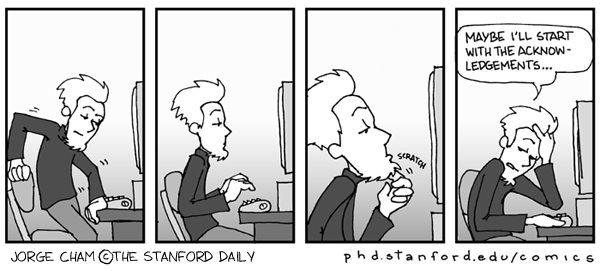
\includegraphics[width=\textwidth]{escrita}
		\fonte{http://www.phdcomics.com/comics/archive.php?comicid=149}
	\end{minipage}
\end{figure}

\subsection{Tabelas}
A Tabela~\ref{tab:estacoes} é um exemplo de tabela elaborada pelo(a) próprio(a) autor(a).

\begin{table}
	\caption{Período das estações do ano no Brasil}
	\label{tab:estacoes}
	\centering%
	\begin{minipage}{.6\textwidth}
		\begin{tabular*}{\textwidth}{ll}
			\hline
			\textbf{Meses} & \textbf{Estações do Ano}\\
			\hline
			21 de março a 21 de junho & Outono\\
			21 de junho a 23 de setembro & Inverno\\
			23 de setembro a 21 de dezembro & Primavera\\
			21 de dezembro a 21 de março & Verão\\
			\hline
		\end{tabular*}
		\fonte{Elaborada pela autora.}
	\end{minipage}
\end{table}

\section{Resumo}
O resumo deve conter de 100 a 500 palavras. No resumo não deve haver citações e indica-se que essa seja a última seção do texto a ser escrita. Veja abaixo uma sugestão de organização e exemplo de resumo de \citetexto{Moro11}.

Sugestão (uma a três linhas para cada item):
\begin{itemize}
	\item Contexto geral e específico;
	\item Questão/problema sendo investigado (propósito do trabalho);
	\item Estado-da-arte (por que precisa de uma solução nova/melhor);
	\item Solução (nome da proposta, metodologia básica sem detalhes, quais características respondem as questões iniciais, interpretação dos resultados, conclusões).
\end{itemize}

Exemplo (SANTOS et al., 2008 apud \citealp{Moro11}):
\begin{quote}
CONTEXTO: A Web é abundante em páginas que armazenam  dados de forma implícita. PROBLEMA: Em muitos casos, estes dados estão presentes em textos semiestruturados sem a presença de delimitadores explícitos e organizados em uma estrutura também implícita. SOLUÇÃO: Este artigo apresenta uma nova abordagem para extração em textos semi-estruturados baseada em Modelos de Markov Ocultos (Hidden Markov Models - HMM). ESTADO-DA-ARTE e MÉTODO PROPOSTO: Ao contrário de outros trabalhos baseados em HMM, a abordagem proposta dá ênfase à extração de metadados, além dos dados propriamente ditos. Esta abordagem consiste no uso de uma estrutura aninhada de HMMs, onde um HMM principal identifica os atributos no texto e HMMs internos, um para cada atributo, identificam os dados e metadados. Os HMMs são gerados a partir de um treinamento com uma fração de amostras da base a ser extraída. RESULTADOS: Os experimentos realizados com anúncios de classificados retirados da Web mostram que o processo de extração alcança qualidade acima de 0,97 com a medida F, mesmo se esta fração de treinamento é pequena. 
\end{quote}

%=======================================================================
% Exemplos de Citações e Referências Bibliográficas
%=======================================================================
\chapter{Exemplos de Citações e Referências Bibliográficas}
\nobibliography* % para usar o \bibentry
Neste capítulo são apresentados exemplos de citações e referências bibliográficas.  Aqui é utilizado o pacote \texttt{bibentry}, que permite a inserção de referências no meio do texto (atenção para a diferença entre citações e referências).

Você vai ver que, neste exemplo, não está sendo usado o estilo de referências bibliográficas do projeto ABNTeX\footnote{http://http://sourceforge.net/projects/abntex}.  Você é completamente livre para usá-lo (veja no início do arquivo .tex como fazer isso).  Os motivos para não usar o ABNTeX neste exemplo são basicamente dois:
\begin{itemize}
	\item Para usar o ABNTeX, é necessário instalá-lo em seu sistema \TeX\ primeiro; embora não seja uma tarefa tão complicada, enxergamos como uma dificuldade a mais para o usuário iniciante.  Nosso objetivo aqui é facilitar ao aluno da UNISINOS o uso deste modelo, de modo que basta copiar os arquivos \texttt{UNISINOSmonografia.cls} e \texttt{unisinos.bst} para a pasta onde estão seus arquivos .tex;
	\item As normas da ABNT são tão complexas que, para atender a todas as variações possíveis de citações e referências, o projeto ABNTeX criou uma série de campos adicionais nas entradas do arquivo .bib.  Embora funcione para o caso ABNT, o efeito colateral de fazer isso é que o seu arquivo .bib será muitas vezes incompatível com os demais estilos tradicionais do BibTeX, como \texttt{plain}, \texttt{alpha}, \texttt{ieeetr}, entre outros.  Por exemplo, em referências a artigos publicados em conferências, o campo \texttt{organization} é usado pelo ABNTeX para definir o nome do evento.  Isso não é padrão e não será reconhecido pelos estilos tradicionais\footnote{Veja como criar seus arquivos .bib no manual do BibTeX, que pode ser encontrado em http://ctan.tug.org/tex-archive/biblio/bibtex/contrib/doc/btxdoc.pdf.}.  Considerando que um dos maiores benefícios do BibTeX é criar um arquivo .bib que pode ser reutilizado pelo resto da vida, nossa estratégia com o \texttt{unisinos.bst} foi tentar aproximar ao máximo a formatação exigida pela ABNT sem implicar na criação de arquivos .bib incompatíveis.  Isso funciona bem na grande maioria dos casos, mas não em todos.  Nesse caso, a saída é usar o ABNTeX ou então alterar manualmente o arquivo .bbl que é gerado ao rodar o comando \texttt{bibtex}.
\end{itemize}

Em caso de dúvida, siga as orientações do manual da Biblioteca \cite{Biblioteca11} e, se necessário, da norma NBR~6023 \cite{NBR6023:2002}.

\section{Artigos em Periódicos}
\begin{itemize}
	\item \bibentry{giallorenzo2021virtualization}.
	\item \bibentry{huong2022development}.
	\item \bibentry{nakajima2011optimizing}.
\end{itemize}

\section{Artigos em Conferências}

\section{Teses e Dissertações}
Seguem algumas referências a trabalhos acadêmicos, como teses, dissertações, trabalhos de conclusão de curso, etc.

%=======================================================================
% Referências
%=======================================================================
\bibliography{referencias}

%=======================================================================
% Exemplo de Apêndice
% O Apêndice é utilizado para apresentar material complementar elaborado
% pelo próprio autor.  Deve seguir as mesmas regras de formatação do
% corpo principal do documento.
%=======================================================================
\appendix
\chapter{Informações Complementares}

O Apêndice é o lugar para incluir textos complementares, que não são essenciais para o entendimento do assunto principal da monografia, mas que podem contribuir com informação relevante (por exemplo, uma prova matemática, uma conceituação básica, etc.).  Ele deve seguir o formato normal do documento.

%=======================================================================
% Exemplo de Anexo
% O Anexo é utilizado para a ``inclusão de materiais não elaborados pelo
% próprio autor, como cópias de artigos, manuais, folders, balancetes, etc.
% e não precisam estar em conformidade com o modelo''.
%=======================================================================
\annex
\chapter{Artigos Publicados}
Existe diferença entre os Apêndices e os Anexos.  Os apêndices trazem informação escrita pelo próprio autor do trabalho, incorporando-se ao formato da monografia como um todo.  Já um anexo é um material à parte, definido/publicado por si só, e que o autor julga conveniente ser apresentado juntamente com a monografia.  Normalmente também vai apresentar formato próprio, como um artigo publicado, um folder, uma planilha, etc.
\end{document}
